\chapter{Projektorganisation}

	\section{Projektteam}
	\begin{figure}[H]
		\begin{minipage}[b]{0.5\linewidth}
			
\includegraphics[width=0.5\textwidth]{projectPlan/media/img/lmurer.jpg}
			\centering
			\caption{Laurin Murer}
			\label{fig:laurinmurer}
		\end{minipage}
		\begin{minipage}[b]{0.5\linewidth}
			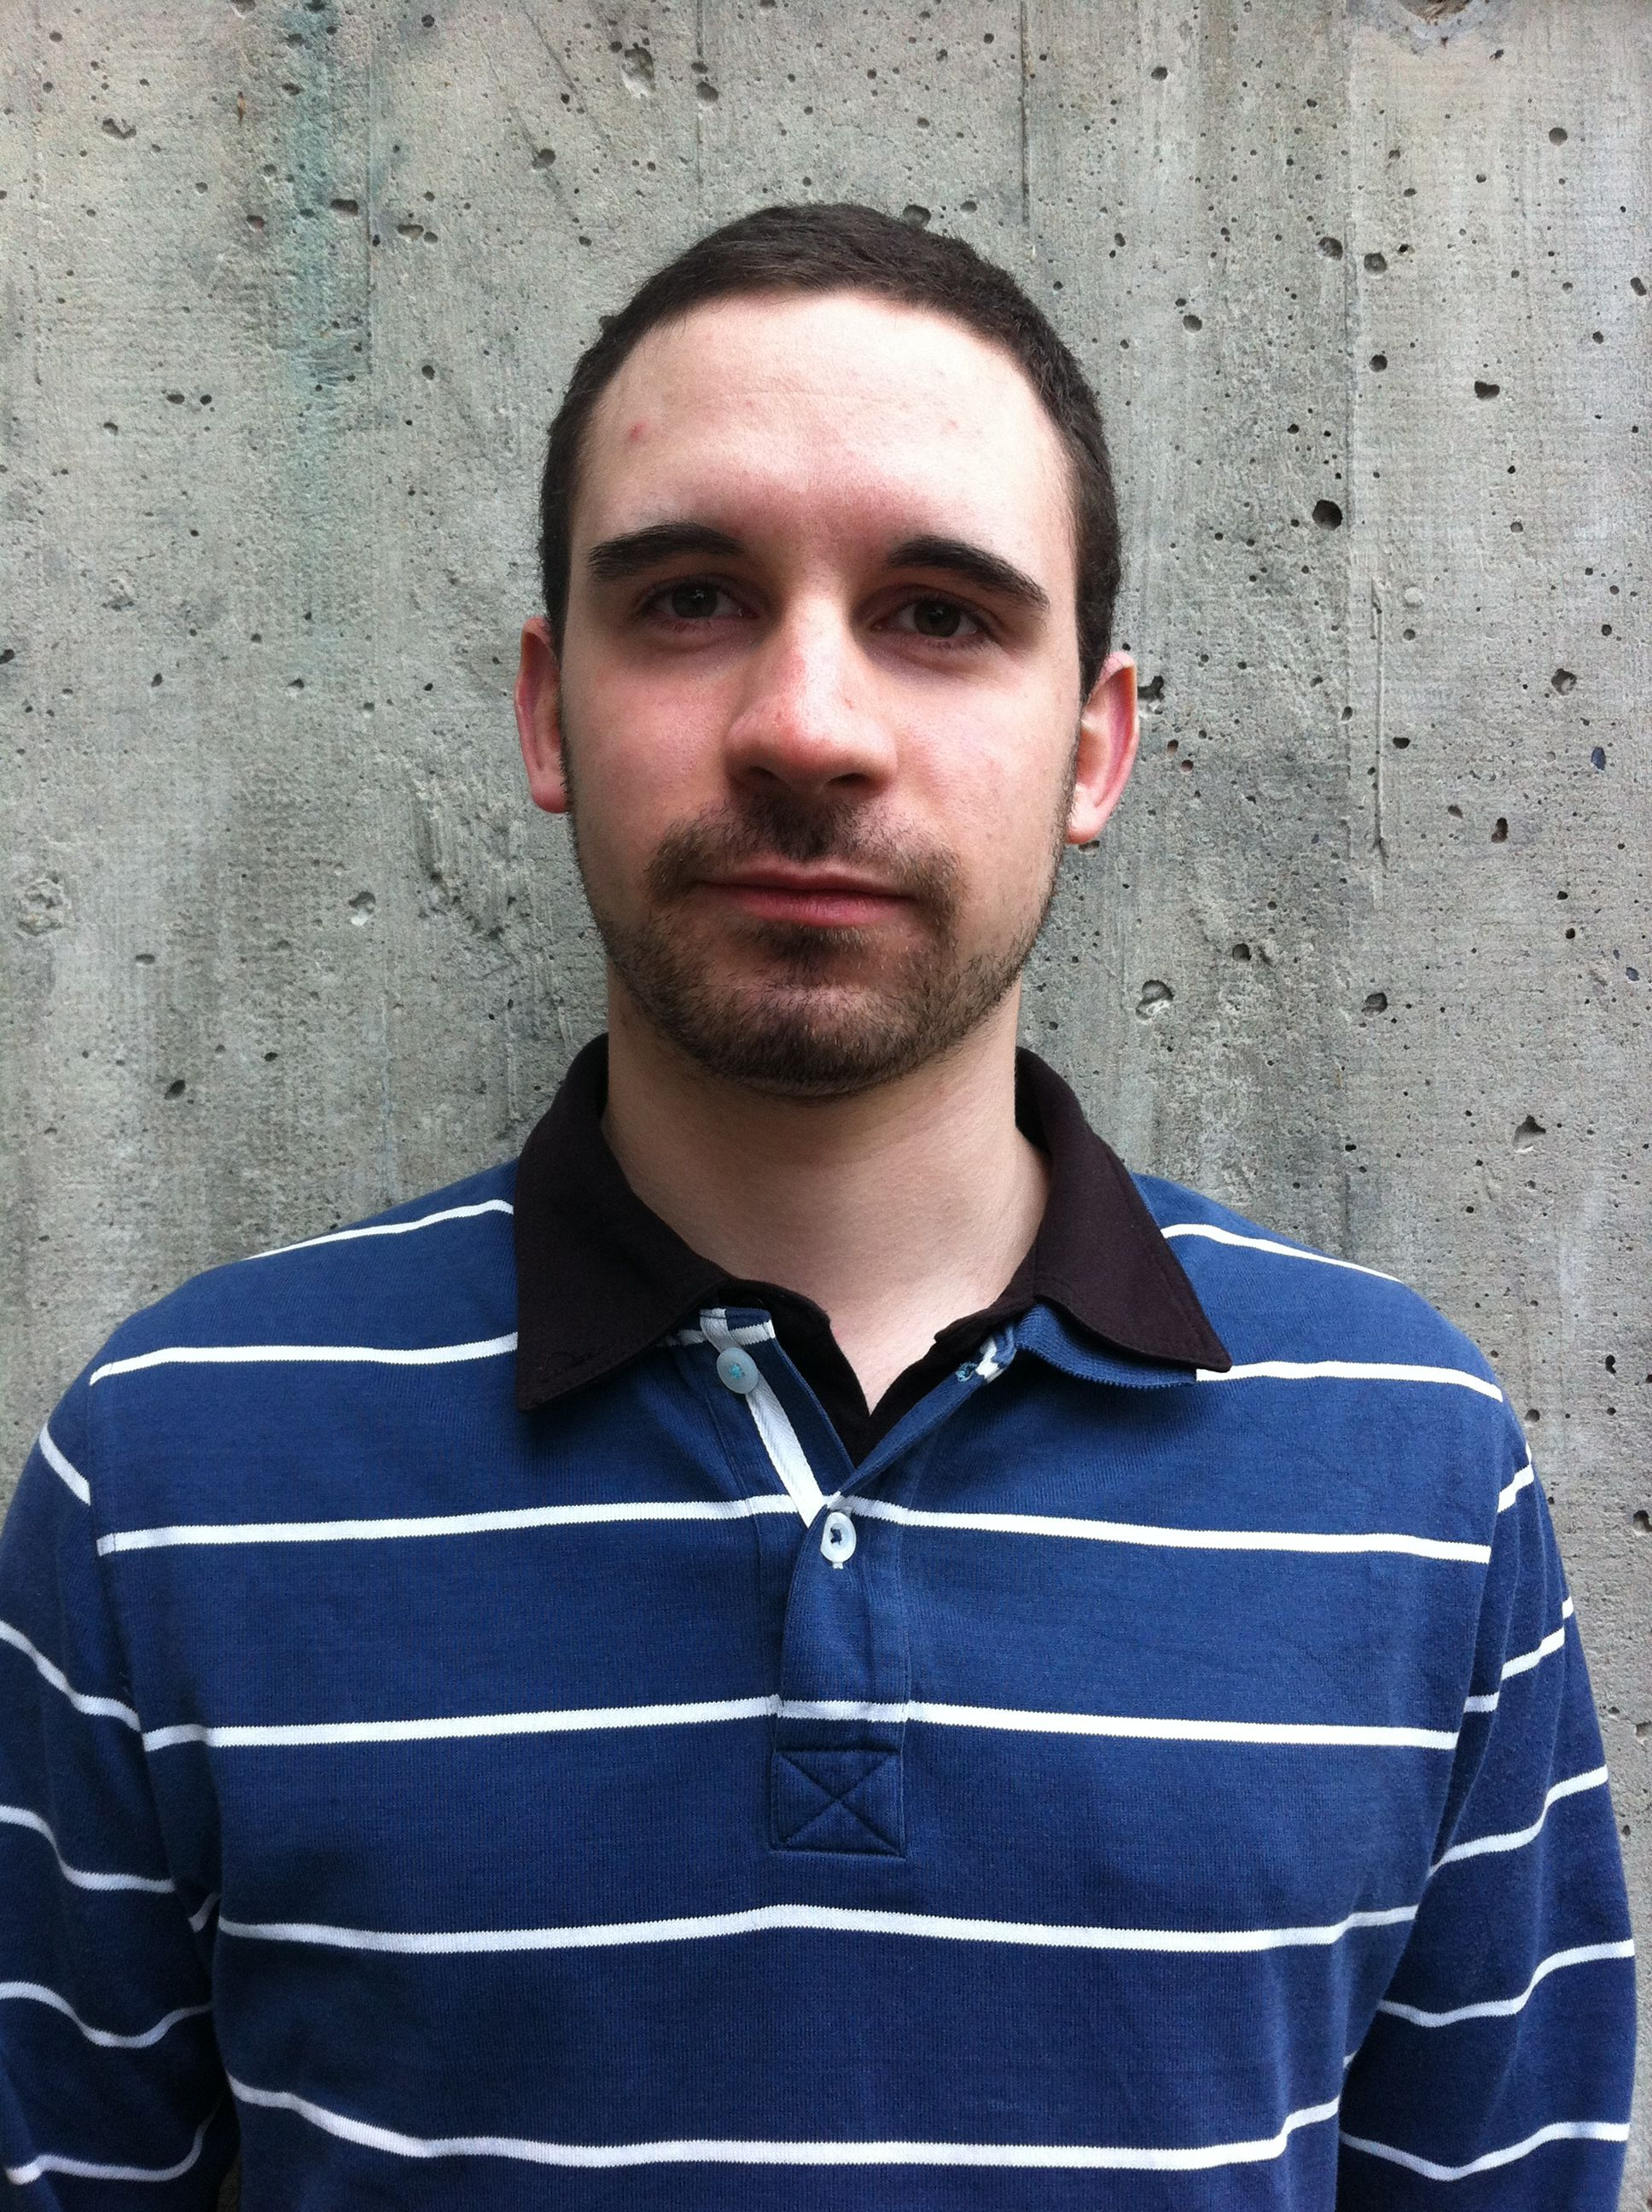
\includegraphics[width=0.5\textwidth]{projectPlan/media/img/tblaser.jpg}
			\centering
			\caption{Tobias Blaser}
			\label{fig:tobiasblaser}
		\end{minipage}
	\end{figure}

	\section{Projektbegleitung}
	\begin{figure}[H]
		\begin{minipage}[b]{0.5\linewidth}
			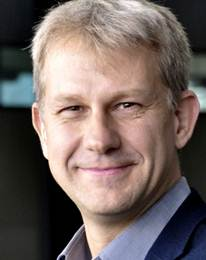
\includegraphics[width=0.5\textwidth]{projectPlan/media/img/ozimmermann.jpg}
			\centering
			\caption{\teacher}
			\label{fig:olafzimmermann}
		\end{minipage}
	\end{figure}
	\teacher\ betreut die Semesterarbeit und begleitet das Team durch regelmässige Meetings.


	\section{Projektmanagement}
		Zur Verwaltung des Projektes hat das Projektteam ein Jira eingesetzt.
		Zur Grobplanung und zur Planung der Milestones wurden Jira-Versions eingesetzt.
		
		\begin{figure}[H]
			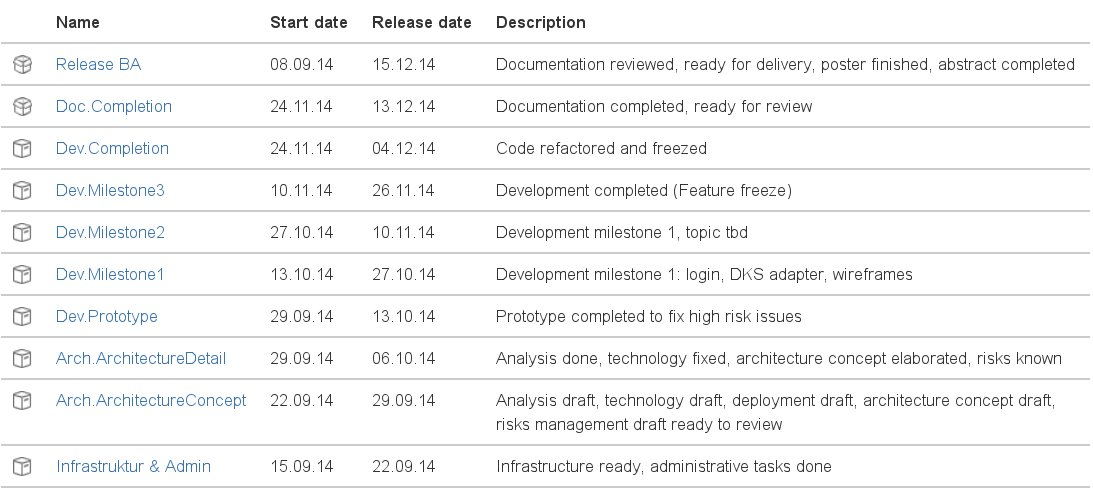
\includegraphics[width=\textwidth]{projectPlan/media/img/jiraVersions.jpg}
			\centering
			\caption{Jira Versions/Milestones}
			\label{fig:jiraVersions}
		\end{figure}
		
		Issues wurden von uns in Zusammenarbeit mit dem Kunden diesen Versionen zugeordnet.
		Zusätzlich haben wir Labels zur Strukturierung eingesetzt.
		
		\begin{figure}[H]
			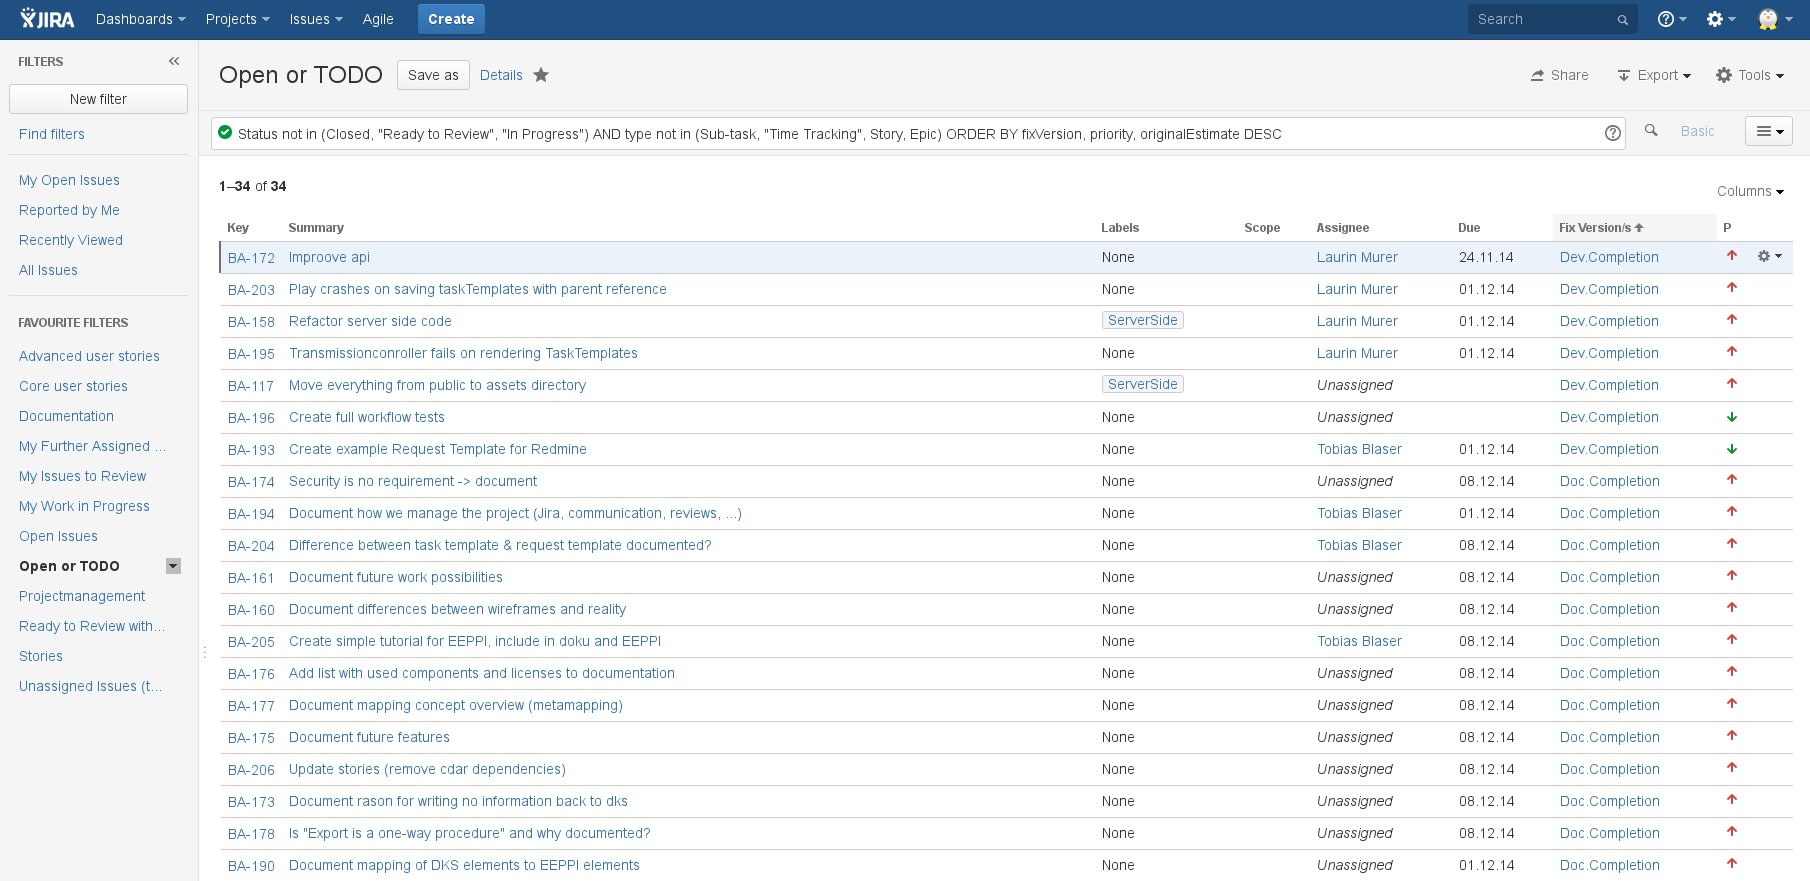
\includegraphics[width=\textwidth]{projectPlan/media/img/jiraIssuesOpenOrTodo.jpg}
			\centering
			\caption{Jira Issues, sortiert nach Version}
			\label{fig:jiraIssuesOpenOrTodo}
		\end{figure}
		
		Mit der Dauer einer Version sowie den geschätzten Aufwänden
		pro Issue haben wir jeweils eine Milestoneplanung durchgeführt.		
		Wir haben jeweils maximal 2/3 der zur Verfügung stehenden Zeit für
		Issues eingeplant und den Rest für Unvorhergesehenes, 
		Meetings und Planung vorgesehen.
		
		\begin{figure}[H]
			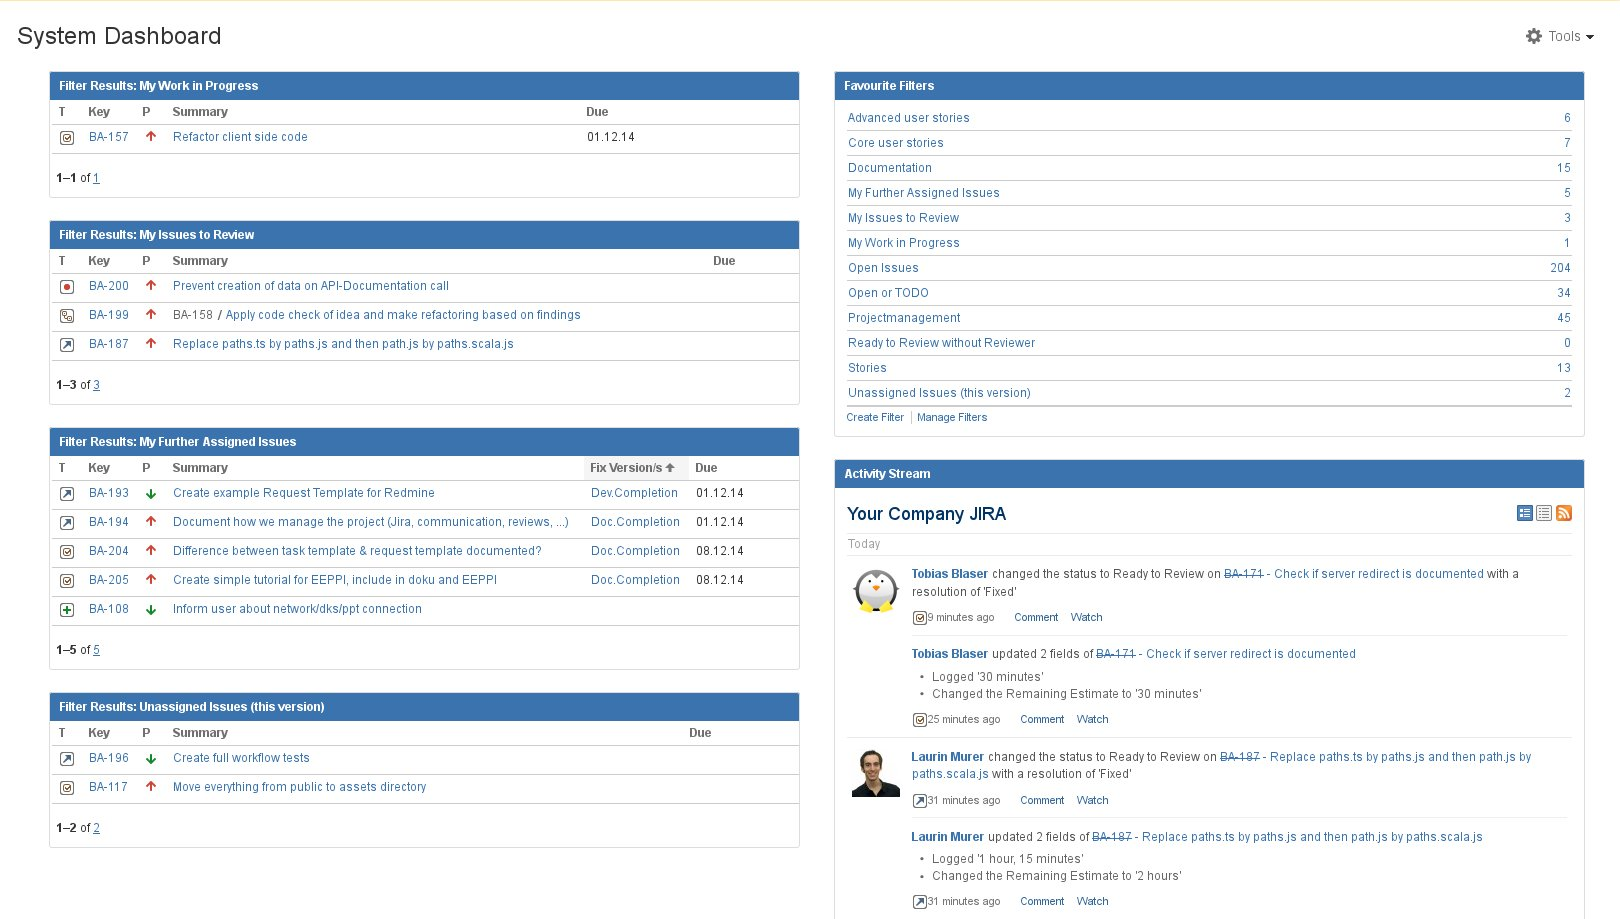
\includegraphics[width=\textwidth]{projectPlan/media/img/jiraDashBoard.jpg}
			\centering
			\caption{Jira Dashboard}
			\label{fig:jiraDashBoard}
		\end{figure}
		
		Jira bietet anpassbare Dashboards, 
		die einen Überblick über das laufende Projekt bieten.
		
		Der Activity Stream von Jira sowie die Git History ermöglichten es uns auf einfache Weise nachzuvollziehen,
		an was der Teampartner in den letzten Stunden gearbeitet hat. 
		Dies senkt den Kommunikationsaufwand und die Notwendigkeit,
		jederzeit gemeinsam an einem Ort zu arbeiten.
		
		\begin{figure}[H]
			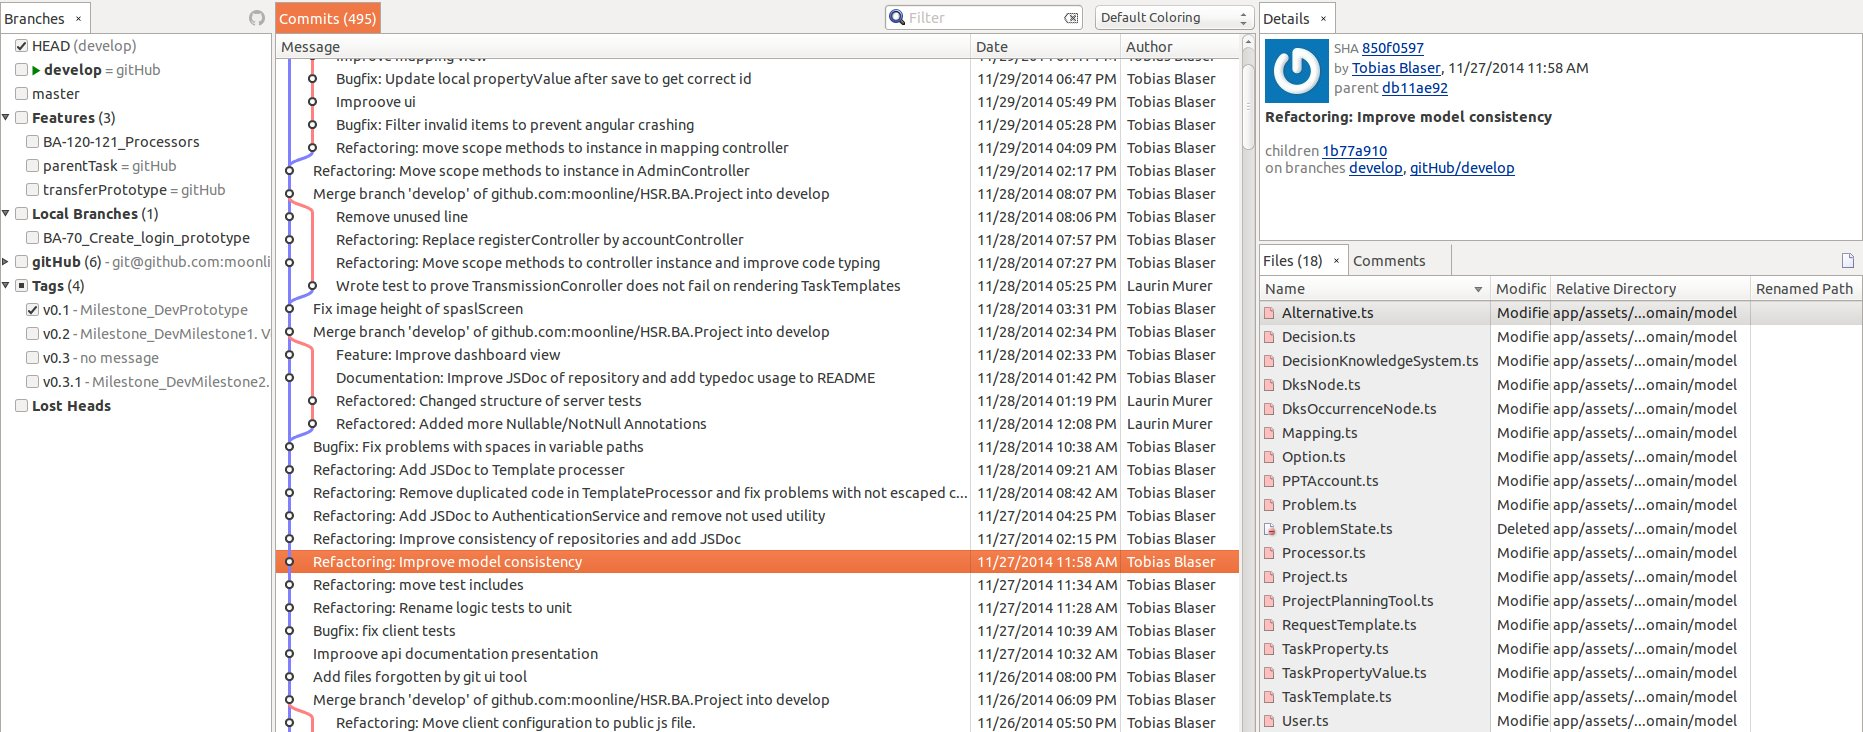
\includegraphics[width=\textwidth]{projectPlan/media/img/gitHistory.jpg}
			\centering
			\caption{Git History}
			\label{fig:gitHistory}
		\end{figure}
		
		Für grössere Features haben wir Git Flow Featurebranches eingesetzt.
		Für Releases entsprechend Releasebranches.
		Zusätzliche haben wir die Funktion "'Releases"' von Github
		zum Hinzufügen von fertigen Builds zu Releases genutzt.
		
		\begin{figure}[H]
			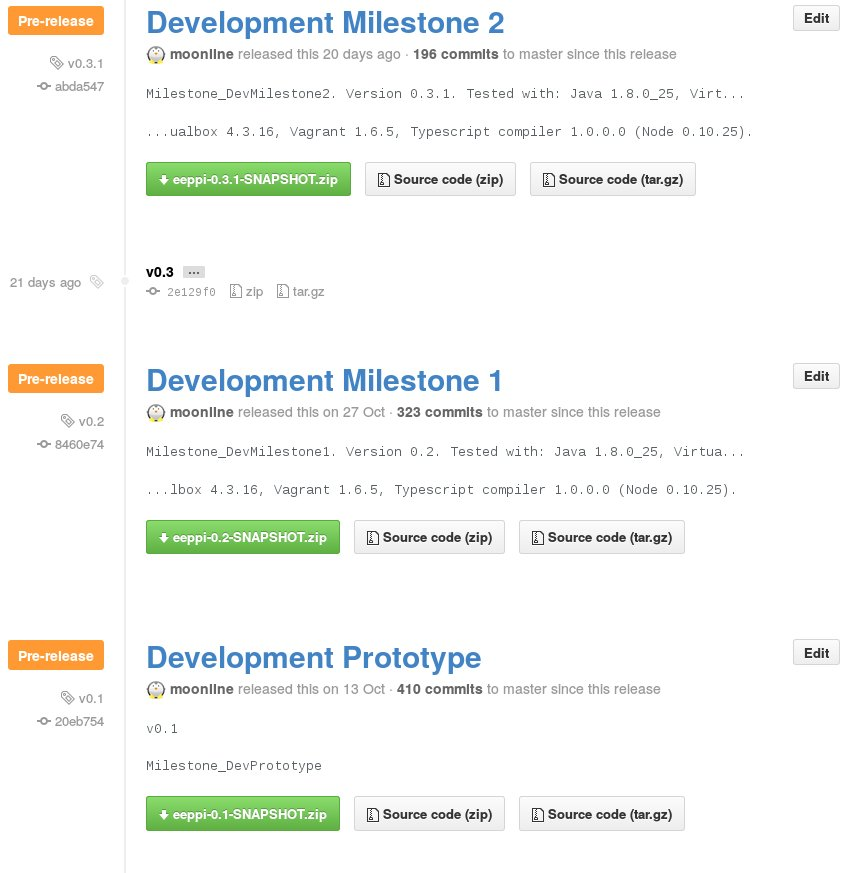
\includegraphics[width=0.5\textwidth]{projectPlan/media/img/githubReleases.jpg}
			\centering
			\caption{Github Releases mit Build-Archives}
			\label{fig:githubReleases}
		\end{figure}

		
	\section{Qualitätssicherung}
		Um sicherzustellen, dass keine Issues geschlossen werden,
		ohne dass die Arbeit einem Review unterzogen wurde,
		haben wir den Issue Workflow im Jira entsprechend gestaltet.		
		
		\begin{figure}[H]
			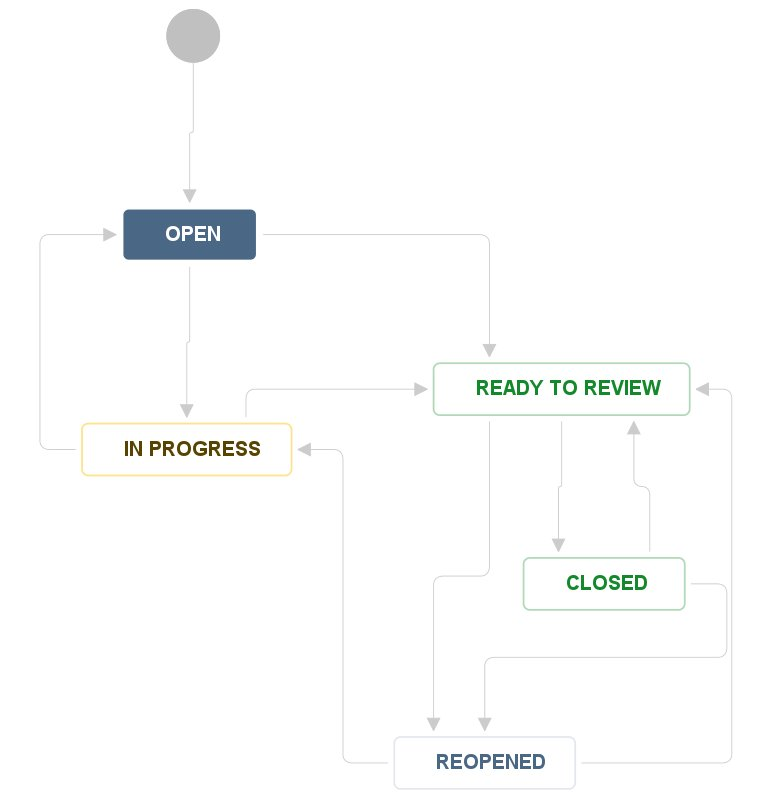
\includegraphics[width=0.5\textwidth]{projectPlan/media/img/jiraIssueWorkflow.jpg}
			\centering
			\caption{Jira Issue Workflow}
			\label{fig:jiraIssueWorkflow}
		\end{figure}
		
		Fertig gestellte Issues müssen immer dem andern Teammitglied
		zum Review gesandt werden und tauchen entsprechend auf dessen
		Dashboard als "'Ready to Review"' auf.
		
		Es geht dabei nicht darum, 
		für jeden erledigten Issue den kompletten Code des Andern anzusehen, 
		sondern das Resultat grob anzuschauen und eventuell
		Edge-Cases\footnote{Spezialfälle, bezogen auf Input Daten oder 
		Workflows der grafischen Oberfläche} zu prüfen. 
		Ein komplettes Code Review jedes Issues wäre zeitlich nicht verhältnismässig.
